\documentclass[UTF8]{ctexart}
\usepackage{listings}
\usepackage{geometry}
\usepackage{titlesec}
\usepackage{booktabs}
\usepackage{multirow}
\usepackage{amsmath}
\usepackage{amssymb}
\usepackage{multicol}
\usepackage{circuitikz}
\usetikzlibrary{arrows,shapes.gates.logic.US,shapes.gates.logic.IEC,calc,quotes,shapes.geometric}
\lstset{numbers=left, basicstyle=\ttfamily}
\geometry{a4paper,left=2.5cm,right=2cm,top=2.5cm,bottom=2cm,headsep=0.5cm}
\linespread{1}

\begin{document}

    \newpagestyle{main}{
    \sethead {第七周} {《计算系统基础》作业} {nyako}
    \setfoot {} {\thepage} {\today}
    \headrule
    \footrule
    }
    \pagestyle{main}
    \paragraph{6.9}
    \begin{center}
        \renewcommand\arraystretch{1.5}
        \begin{tabular}{r@{}c@{}l@{}}
            \texttt{11001100 AND 01010101}&\texttt { =}&\texttt{ 0100 0100}\\
            \texttt{(1100 AND 0101) AND 1101}&\texttt { =}&\texttt{ 0100}\\
            \texttt{1100 AND (0101 AND 1101)}&\texttt { =}&\texttt{ 0100}\\
            \texttt{11001100 OR 01010101}&\texttt { =}&\texttt{ 1101 1101}\\
            \texttt{(1100 OR 0101) OR 1101}&\texttt { =}&\texttt{ 1101}\\
            \texttt{1100 OR (0101 OR 1101)}&\texttt { =}&\texttt{ 1101}\\
            \texttt{NOT(NOT 1011)}&\texttt { =}&\texttt{ 1011}\\
            \texttt{1101 XOR 0101}&\texttt { =}&\texttt{ 1000}\\
            \texttt{NOT((NOT 1101) OR (NOT 0101))}&\texttt { =}&\texttt{ 0101}\\
            \texttt{NOT((NOT 1101) AND (NOT 0101))}&\texttt { =}&\texttt{ 1101}\\
            \texttt{((NOT 1101) AND 0101) OR (1101 AND (NOT 0101))}&\texttt { =}&\texttt{ 1000}\\
        \end{tabular}
    \end{center}
    \paragraph{6.16} 从键盘读入一个整数,输出其二进制表示下 $1$ 的个数.
    \paragraph{7.1}1).
    \begin{center}
        \begin{multicols}{2}
            \setlength{\columnseprule}{1pt}
            三输入与门\\\bigskip
            \begin{circuitikz}[scale=.8]
                \draw (0,0) node[pmos, emptycircle](pmos1) {}
                (pmos1.base) node[anchor=east] {$A$}
                (pmos1.collector) node {}
                (pmos1.emitter) node {}
                (0,1)node[rground, yscale=-1](){} -- (pmos1.emitter)
                (2,0) node[pmos, emptycircle](pmos2) {}
                (pmos2.base) node[anchor=east] {$B$}
                (pmos2.collector) node {}
                (pmos2.emitter) node {}
                (2,1)node[rground, yscale=-1](){} -- (pmos2.emitter)
                (4,0) node[pmos, emptycircle](pmos3) {}
                (pmos3.base) node[anchor=east] {$C$}
                (pmos3.collector) node {}
                (pmos3.emitter) node {}
                (4,1)node[rground, yscale=-1](){} -- (pmos3.emitter)
                (2,-3) node[nmos, emptycircle](nmos1) {}
                (nmos1.base) node[anchor=east] {$A$}
                (nmos1.collector) node {}
                (nmos1.emitter) node {}
                (2,-5) node[nmos, emptycircle](nmos2) {}
                (nmos2.base) node[anchor=east] {$B$}
                (nmos2.collector) node {}
                (nmos2.emitter) node {}
                (2,-7) node[nmos, emptycircle](nmos3) {}
                (nmos3.base) node[anchor=east] {$C$}
                (nmos3.collector) node {}
                (nmos3.emitter) node {}
                (nmos3.collector) -- (nmos2.emitter)
                (nmos2.collector) -- (nmos1.emitter)
                (2,-8)node[rground](){} -- (nmos3.emitter)
                (0,-1) -- (pmos1.collector)
                (2,-1) -- (pmos2.collector)
                (4,-1) -- (pmos3.collector)
                (0,-1) to[short,-*] (2,-1) -- (4,-1)
                (2,-1) -- (nmos1.collector)
                (6,-1) node[pmos, emptycircle](pmos4) {}
                (pmos4.base) node {}
                (pmos4.collector) node {}
                (pmos4.emitter) node {}
                (pmos4) ++(0,1)node[rground, yscale=-1](){} -- (pmos4.emitter)
                (6,-3) node[nmos](nmos4) {}
                (nmos4.base) node {}
                (nmos4.collector) node {}
                (nmos4.emitter) node {}
                (nmos4) ++(0,-1)node[rground](){} -- (nmos4.emitter)
                (pmos4.base) ++(0,-1) -- (2, -2)
                (pmos4.base) -- (nmos4.base)
                (pmos4.collector) -- (nmos4.collector)
                (6,-2) --++(1,0) node[anchor=west]{$OUT$}
                ;
            \end{circuitikz}
            
            \vfill\null
            \columnbreak

            三输入或门\\\bigskip
            \begin{circuitikz}[scale=.8]
                \draw (0,-7) node[nmos, emptycircle](nmos1) {}
                (nmos1.base) node[anchor=east] {$A$}
                (nmos1.collector) node {}
                (nmos1.emitter) node {}
                (0,-8)node[rground](){} -- (nmos1.emitter)
                (2,-7) node[nmos, emptycircle](nmos2) {}
                (nmos2.base) node[anchor=east] {$B$}
                (nmos2.collector) node {}
                (nmos2.emitter) node {}
                (2,-8)node[rground](){} -- (nmos2.emitter)
                (4,-7) node[nmos, emptycircle](nmos3) {}
                (nmos3.base) node[anchor=east] {$C$}
                (nmos3.collector) node {}
                (nmos3.emitter) node {}
                (4,-8)node[rground](){} -- (nmos3.emitter)
                (2,0) node[pmos, emptycircle](pmos1) {}
                (pmos1.base) node[anchor=east] {$A$}
                (pmos1.collector) node {}
                (pmos1.emitter) node {}
                (2,-2) node[pmos, emptycircle](pmos2) {}
                (pmos2.base) node[anchor=east] {$B$}
                (pmos2.collector) node {}
                (pmos2.emitter) node {}
                (2,-4) node[pmos, emptycircle](pmos3) {}
                (pmos3.base) node[anchor=east] {$C$}
                (pmos3.collector) node {}
                (pmos3.emitter) node {}
                (2,1)node[rground, yscale=-1](){} -- (pmos1.emitter)
                (0,-6) -- (nmos1.collector)
                (2,-6) -- (nmos2.collector)
                (4,-6) -- (nmos3.collector)
                (0,-6) to[short,-*] (2,-6) -- (4,-6)
                (2,-6) -- (pmos3.collector)
                (pmos3.emitter) -- (pmos2.collector)
                (pmos2.emitter) -- (pmos1.collector)
                (6,-4) node[pmos, emptycircle](pmos4) {}
                (pmos4.base) node {}
                (pmos4.collector) node {}
                (pmos4.emitter) node {}
                (pmos4) ++(0,1)node[rground, yscale=-1](){} -- (pmos4.emitter)
                (6,-6) node[nmos](nmos4) {}
                (nmos4.base) node {}
                (nmos4.collector) node {}
                (nmos4.emitter) node {}
                (nmos4) ++(0,-1)node[rground](){} -- (nmos4.emitter)
                (pmos4.base) ++(0,-1) -- (2, -5)
                (pmos4.base) -- (nmos4.base)
                (pmos4.collector) -- (nmos4.collector)
                (6,-5) -- ++(1,0) node[anchor=west]{$OUT$}
                ;
            \end{circuitikz}
        \end{multicols}
    \end{center}
\newpage

    2). $A=0,B=0,C=1$时,
    \begin{center}
        \begin{multicols}{2}
            \setlength{\columnseprule}{1pt}
            三输入与门\\\bigskip
            \begin{circuitikz}[scale=.8]
                \draw
                (0,1)node[rground, yscale=-1](){} -- (0,-1)
                (2,1)node[rground, yscale=-1](){} -- (2,-1)
                (4,1)node[rground, yscale=-1](){} -- (4,-1)
                (0,0) --++(-0.75,0) node[anchor=east] {$0$}
                (2,0) --++(-0.75,0) node[anchor=east] {$0$}
                (4,0) --++(-0.75,0) node[anchor=east] {$1$}
                (2,-3) --++(-0.75,0) node[anchor=east] {$0$}
                (2,-5) --++(-0.75,0) node[anchor=east] {$0$}
                (2,-7) --++(-0.75,0) node[anchor=east] {$1$}
                (0,-1) to[short,-*] (2,-1) -- (4,-1)
                (2,-2)to  node[anchor=south] {$1$} (5,-2)
                (5,-2)|-(6,-1)
                (5,-2)|-(6,-3)
                (6,0)node[rground, yscale=-1](){} -- ++(0,-2)
                (6,-4)node[rground](){} -- ++(0,2)
                (6,-2) --++(1,0) node[anchor=west]{$0$}
                (2,-8)node[rground](){} -- (2,-1)
                ;
                \begin{scope}
                    \clip (0,0) circle (12pt);
                    \draw[dashed,fill=white,line width=0.6pt] (0,0) circle (12pt);
                    \draw[line width=1.5pt] (0,-1) -- (0,1);
                \end{scope}
                ;
                \begin{scope}
                    \clip (2,0) circle (12pt);
                    \draw[dashed,fill=white,line width=0.6pt] (2,0) circle (12pt);
                    \draw[line width=1.5pt] (2,-1) -- (2,1);
                \end{scope}
                ;
                \begin{scope}
                    \clip (4,0) circle (12pt);
                    \draw[dashed,fill=white,line width=0.6pt] (4,0) circle (12pt);
                \end{scope}
                ;
                \begin{scope}
                    \clip (2,-3) circle (12pt);
                    \draw[dashed,fill=white,line width=0.6pt] (2,-3) circle (12pt);
                \end{scope}
                ;
                \begin{scope}
                    \clip (2,-5) circle (12pt);
                    \draw[dashed,fill=white,line width=0.6pt] (2,-5) circle (12pt);
                \end{scope}
                ;
                \begin{scope}
                    \clip (2,-7) circle (12pt);
                    \draw[dashed,fill=white,line width=0.6pt] (2,-7) circle (12pt);
                    \draw[line width=1.5pt] (2,-6) -- (2,-8);
                \end{scope}
                ;
                \begin{scope}
                    \clip (6,-1) circle (12pt);
                    \draw[dashed,fill=white,line width=0.6pt] (6,-1) circle (12pt);
                \end{scope}
                ;
                \begin{scope}
                    \clip (6,-3) circle (12pt);
                    \draw[dashed,fill=white,line width=0.6pt] (6,-3) circle (12pt);
                    \draw[line width=1.5pt] (6,-2) -- (6,-4);
                \end{scope}
                ;

            \end{circuitikz}
            \vfill\null
            \columnbreak

            三输入或门\\\bigskip
            \begin{circuitikz}[yscale=-1,scale=.8]
                \draw
                (0,1)node[rground](){} -- (0,-1)
                (2,1)node[rground](){} -- (2,-1)
                (4,1)node[rground](){} -- (4,-1)
                (0,0) --++(-0.75,0) node[anchor=east] {$0$}
                (2,0) --++(-0.75,0) node[anchor=east] {$0$}
                (4,0) --++(-0.75,0) node[anchor=east] {$1$}
                (2,-3) --++(-0.75,0) node[anchor=east] {$1$}
                (2,-5) --++(-0.75,0) node[anchor=east] {$0$}
                (2,-7) --++(-0.75,0) node[anchor=east] {$0$}
                (0,-1) to[short,-*] (2,-1) -- (4,-1)
                (2,-2)to  node[anchor=south] {$0$} (5,-2)
                (5,-2)|-(6,-1)
                (5,-2)|-(6,-3)
                (6,0)node[rground](){} -- ++(0,-2)
                (6,-4)node[rground, yscale=-1](){} -- ++(0,2)
                (6,-2) --++(1,0) node[anchor=west]{$1$}
                (2,-8)node[rground, yscale=-1](){} -- (2,-1)
                ;
                \begin{scope}
                    \clip (0,0) circle (12pt);
                    \draw[dashed,fill=white,line width=0.6pt] (0,0) circle (12pt);
                \end{scope}
                ;
                \begin{scope}
                    \clip (2,0) circle (12pt);
                    \draw[dashed,fill=white,line width=0.6pt] (2,0) circle (12pt);
                \end{scope}
                ;
                \begin{scope}
                    \clip (4,0) circle (12pt);
                    \draw[dashed,fill=white,line width=0.6pt] (4,0) circle (12pt);
                    \draw[line width=1.5pt] (4,-1) -- (4,1);
                \end{scope}
                ;
                \begin{scope}
                    \clip (2,-3) circle (12pt);
                    \draw[dashed,fill=white,line width=0.6pt] (2,-3) circle (12pt);
                \end{scope}
                ;
                \begin{scope}
                    \clip (2,-5) circle (12pt);
                    \draw[dashed,fill=white,line width=0.6pt] (2,-5) circle (12pt);
                    \draw[line width=1.5pt] (2,-4) -- (2,-6);
                \end{scope}
                ;
                \begin{scope}
                    \clip (2,-7) circle (12pt);
                    \draw[dashed,fill=white,line width=0.6pt] (2,-7) circle (12pt);
                    \draw[line width=1.5pt] (2,-6) -- (2,-8);
                \end{scope}
                ;
                \begin{scope}
                    \clip (6,-1) circle (12pt);
                    \draw[dashed,fill=white,line width=0.6pt] (6,-1) circle (12pt);
                \end{scope}
                ;
                \begin{scope}
                    \clip (6,-3) circle (12pt);
                    \draw[dashed,fill=white,line width=0.6pt] (6,-3) circle (12pt);
                    \draw[line width=1.5pt] (6,-2) -- (6,-4);
                \end{scope}
                ;
            \end{circuitikz}
        \end{multicols}
    \end{center}
    \paragraph{7.2}1).
    \begin{center}
        \begin{tabular}{ccc|c}
            \toprule
            $A$&$B$&$C$&$D$\\
            \midrule
            0&0&0&1\\
            0&0&1&1\\
            0&1&0&1\\
            0&1&1&0\\
            1&0&0&1\\
            1&0&1&0\\
            1&1&0&1\\
            1&1&1&0\\
            \bottomrule
        \end{tabular}
    \end{center}
    2).
    \begin{center}
        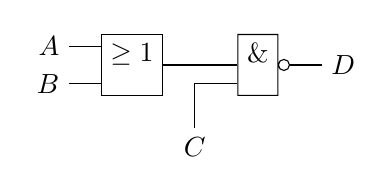
\begin{tikzpicture}[scale=.8]
            \node[or gate IEC, draw, logic gate inputs=nnnn] at (0,0) (a) {};
            \node[nand gate IEC, draw, logic gate inputs=nnnn] at (2,0) (o) {};
            \draw (a.input 1)--++(-0.5,0) node[anchor=east] {$A$}
            (a.output)--(o.input 1 |- a.output)
            (a.input 4)--++(-0.5,0) node[anchor=east] {$B$}
            (o.input 4)-|(1,-1) node[anchor=north] {$C$}
            (o.output) -- ++(0.5,0) node[anchor=west]{$D$}
            ;
        \end{tikzpicture}
    \end{center}
    \paragraph{7.3} $A,B$输入相反时,将导致短路.
    \newpage
    \paragraph{7.4}
    \begin{center}
        \begin{tikzpicture}
            \node[and gate IEC, draw, logic gate inputs=iiii] at (0,0) (a1) {};
            \node[and gate IEC, draw, logic gate inputs=iiin] at ($(a1)+(0,-1)$) (a2) {};
            \node[and gate IEC, draw, logic gate inputs=iini] at ($(a2)+(0,-1)$) (a3) {};
            \node[and gate IEC, draw, logic gate inputs=iinn] at ($(a3)+(0,-1)$) (a4) {};
            \node[and gate IEC, draw, logic gate inputs=inii] at ($(a4)+(0,-1)$) (a5) {};
            \node[and gate IEC, draw, logic gate inputs=inin] at ($(a5)+(0,-1)$) (a6) {};
            \node[and gate IEC, draw, logic gate inputs=inni] at ($(a6)+(0,-1)$) (a7) {};
            \node[and gate IEC, draw, logic gate inputs=innn] at ($(a7)+(0,-1)$) (a8) {};
            \node[and gate IEC, draw, logic gate inputs=niii] at ($(a8)+(0,-1)$) (a9) {};
            \node[and gate IEC, draw, logic gate inputs=niin] at ($(a9)+(0,-1)$) (a10) {};
            \node[and gate IEC, draw, logic gate inputs=nini] at ($(a10)+(0,-1)$) (a11) {};
            \node[and gate IEC, draw, logic gate inputs=ninn] at ($(a11)+(0,-1)$) (a12) {};
            \node[and gate IEC, draw, logic gate inputs=nnii] at ($(a12)+(0,-1)$) (a13) {};
            \node[and gate IEC, draw, logic gate inputs=nnin] at ($(a13)+(0,-1)$) (a14) {};
            \node[and gate IEC, draw, logic gate inputs=nnni] at ($(a14)+(0,-1)$) (a15) {};
            \node[and gate IEC, draw, logic gate inputs=nnnn] at ($(a15)+(0,-1)$) (a16) {};
            \foreach \n in {1,...,4}
            \node (c\n) at ($ (\n/4-2,0) $) {};
            \node (d) at (-2.5,0) {};
            \foreach \m in {2,...,15}
            \foreach \n in {1,...,4}
            \draw (a\m.input \n) to [short, -*] (c\n |- a\m.input \n);
            \foreach \n in {1,...,4}{
            \draw (a1.input \n) to (c\n |- a1.input \n);
            \draw (a16.input \n) -| (c\n |- a1.input \n);
            }
            \draw (c1 |- a1.input 1) to (d |- a1.input 1) node[anchor=east]{$A$};
            \draw (c2 |- a2.input 2) -- (d |- a2.input 2) node[anchor=east]{$B$};
            \draw (c3 |- a3.input 3) -- (d |- a3.input 3) node[anchor=east]{$C$};
            \draw (c4 |- a4.input 4) -- (d |- a4.input 4) node[anchor=east]{$D$};
            \draw (a1.output) -- ++(1,0) node[anchor=west]{$1,\text{ 当\ } A,B,C,D\text{ 为\ } 0000\text{ 时}$};
            \draw (a2.output) -- ++(1,0) node[anchor=west]{$1,\text{ 当\ } A,B,C,D\text{ 为\ } 0001\text{ 时}$};
            \draw (a3.output) -- ++(1,0) node[anchor=west]{$1,\text{ 当\ } A,B,C,D\text{ 为\ } 0010\text{ 时}$};
            \draw (a4.output) -- ++(1,0) node[anchor=west]{$1,\text{ 当\ } A,B,C,D\text{ 为\ } 0011\text{ 时}$};
            \draw (a5.output) -- ++(1,0) node[anchor=west]{$1,\text{ 当\ } A,B,C,D\text{ 为\ } 0100\text{ 时}$};
            \draw (a6.output) -- ++(1,0) node[anchor=west]{$1,\text{ 当\ } A,B,C,D\text{ 为\ } 0101\text{ 时}$};
            \draw (a7.output) -- ++(1,0) node[anchor=west]{$1,\text{ 当\ } A,B,C,D\text{ 为\ } 0110\text{ 时}$};
            \draw (a8.output) -- ++(1,0) node[anchor=west]{$1,\text{ 当\ } A,B,C,D\text{ 为\ } 0111\text{ 时}$};
            \draw (a9.output) -- ++(1,0) node[anchor=west]{$1,\text{ 当\ } A,B,C,D\text{ 为\ } 1000\text{ 时}$};
            \draw (a10.output) -- ++(1,0) node[anchor=west]{$1,\text{ 当\ } A,B,C,D\text{ 为\ } 1001\text{ 时}$};
            \draw (a11.output) -- ++(1,0) node[anchor=west]{$1,\text{ 当\ } A,B,C,D\text{ 为\ } 1010\text{ 时}$};
            \draw (a12.output) -- ++(1,0) node[anchor=west]{$1,\text{ 当\ } A,B,C,D\text{ 为\ } 1011\text{ 时}$};
            \draw (a13.output) -- ++(1,0) node[anchor=west]{$1,\text{ 当\ } A,B,C,D\text{ 为\ } 1100\text{ 时}$};
            \draw (a14.output) -- ++(1,0) node[anchor=west]{$1,\text{ 当\ } A,B,C,D\text{ 为\ } 1101\text{ 时}$};
            \draw (a15.output) -- ++(1,0) node[anchor=west]{$1,\text{ 当\ } A,B,C,D\text{ 为\ } 1110\text{ 时}$};
            \draw (a16.output) -- ++(1,0) node[anchor=west]{$1,\text{ 当\ } A,B,C,D\text{ 为\ } 1111\text{ 时}$};
        \end{tikzpicture}
    \end{center}
    \newpage
    \paragraph{7.5}
    \begin{center}
        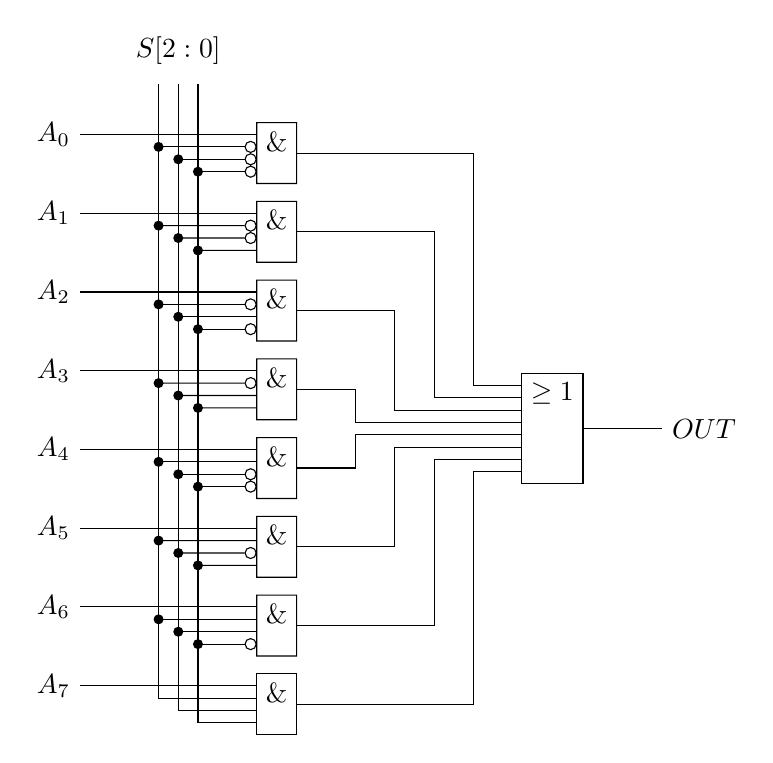
\begin{tikzpicture}
            \node[and gate IEC, draw, logic gate inputs=niii] at (0,0) (a0) {};
            \node[and gate IEC, draw, logic gate inputs=niin] at ($(a0)+(0,-1)$) (a1) {};
            \node[and gate IEC, draw, logic gate inputs=nini] at ($(a1)+(0,-1)$) (a2) {};
            \node[and gate IEC, draw, logic gate inputs=ninn] at ($(a2)+(0,-1)$) (a3) {};
            \node[and gate IEC, draw, logic gate inputs=nnii] at ($(a3)+(0,-1)$) (a4) {};
            \node[and gate IEC, draw, logic gate inputs=nnin] at ($(a4)+(0,-1)$) (a5) {};
            \node[and gate IEC, draw, logic gate inputs=nnni] at ($(a5)+(0,-1)$) (a6) {};
            \node[and gate IEC, draw, logic gate inputs=nnnn] at ($(a6)+(0,-1)$) (a7) {};
            \node[or gate IEC, draw, logic gate inputs=nnnnnnnn] at (3.5,-3.5) (or) {};
            \foreach \n in {1,...,4}
            \node (c\n) at ($ (\n/4-2,1) $) {};
            \node (d) at (-2.5,0) {};
            \node (e1) at (2.5,0) {};
            \node (e2) at (2,0) {};
            \node (e3) at (1.5,0) {};
            \node (e4) at (1,0) {};
            \foreach \m in {0,...,6}
            \foreach \n in {2,...,4}
            \draw (a\m.input \n) to [short, -*] (c\n |- a\m.input \n);
            \foreach \n in {2,...,4}
            \draw (a0.input \n) to (c\n |- a0.input \n);
            \draw (a7.input 2) -| (c2);
            \draw (a7.input 3) -| (c3) node[anchor=south]{$S[2:0]$};
            \draw (a7.input 4) -| (c4);
            \foreach \m in {0,...,7}
            \draw (a\m.input 1) -- (d |- a\m.input 1) node[anchor=east]{$A_\m$};
            \draw (a0.output) -- (e1 |- a0.output) |- (or.input 1);
            \draw (a1.output) -- (e2 |- a1.output) |- (or.input 2);
            \draw (a2.output) -- (e3 |- a2.output) |- (or.input 3);
            \draw (a3.output) -- (e4 |- a3.output) |- (or.input 4);
            \draw (a4.output) -- (e4 |- a4.output) |- (or.input 5);
            \draw (a5.output) -- (e3 |- a5.output) |- (or.input 6);
            \draw (a6.output) -- (e2 |- a6.output) |- (or.input 7);
            \draw (a7.output) -- (e1 |- a7.output) |- (or.input 8);
            \draw (or.output) -- ++(1,0) node[anchor=west]{$OUT$};
        \end{tikzpicture}
    \end{center}
    \paragraph{7.7}
    \[X=\left(\overline{A}\cdot\overline{B}\cdot\overline{C}\right)+\left(\overline{A}\cdot B\cdot\overline{C}\right)+\left(A\cdot\overline{B}\cdot\overline{C}\right)=\overline{A\cdot B+C}\]
    \begin{center}
        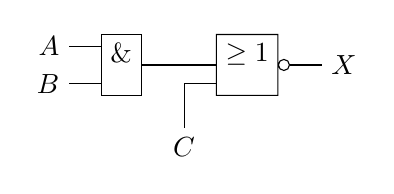
\begin{tikzpicture}[scale=.8]
            \node[and gate IEC, draw, logic gate inputs=nnnn] at (0,0) (a) {};
            \node[nor gate IEC, draw, logic gate inputs=nnnn] at (2,0) (o) {};
            \draw (a.input 1)--++(-0.5,0) node[anchor=east] {$A$}
            (a.output)--(o.input 1|-a.output)
            (a.input 4)--++(-0.5,0) node[anchor=east] {$B$}
            (o.input 4)-|(1,-1) node[anchor=north] {$C$}
            (o.output) -- ++(0.5,0) node[anchor=west]{$X$}
            ;
        \end{tikzpicture}
    \end{center}
    \paragraph{7.8}
    \begin{center}
        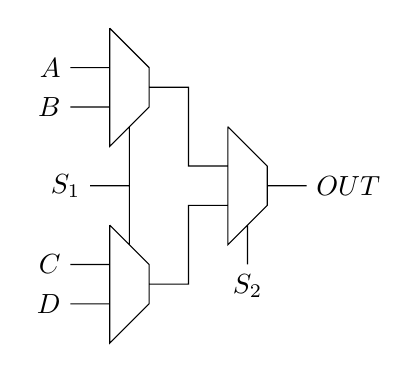
\begin{tikzpicture}
            \draw(0,0)--++(-0.5,0) node[anchor=east]{$A$}
            (0,-0.5)--++(-0.5,0) node[anchor=east]{$B$}
            (0,-2.5)--++(-0.5,0) node[anchor=east]{$C$}
            (0,-3)--++(-0.5,0) node[anchor=east]{$D$}
            (0,0.5)--(0,-1)--(0.5,-0.5)--(0.5,0)--(0,0.5)
            (0,-2)--(0,-3.5)--(0.5,-3)--(0.5,-2.5)--(0,-2)
            (1.5,-0.75)--(1.5,-2.25)--(2,-1.75)--(2,-1.25)--(1.5,-0.75)
            (0.5,-0.25) --+(0.5,0)|- (1.5,-1.25)
            (0.5,-2.75) --+(0.5,0)|- (1.5,-1.75)
            (1.75,-2)--++(0,-0.5) node[anchor=north]{$S_2$}
            (0.25, -0.75) --+ (0, -1.5)
            (0.25,-1.5)--++(-0.5,0) node[anchor=east]{$S_1$}
            (2,-1.5) --+(0.5,0)  node[anchor=west]{$OUT$}
            ;
        \end{tikzpicture}
    \end{center}
    \paragraph{7.9}
    \begin{center}
        \begin{tabular}{ccc|c}
            \toprule
            $A$&$B$&$C$&$D$\\
            \midrule
            0&0&0&0\\
            0&0&1&0\\
            0&1&0&1\\
            0&1&1&0\\
            1&0&0&0\\
            1&0&1&1\\
            1&1&0&1\\
            1&1&1&1\\
            \bottomrule
        \end{tabular}
    \end{center}
    \paragraph{7.10}
    在原电路中,$X=0$和$X=1$时,分别输出$A+B+\text{最右进位}$与$A+C+\text{最右进位}$的值.
    \begin{center}
        \begin{tikzpicture}
            \node (e) at (0,0.75) {};
            \node (d) at (0,1.25) {};
            \foreach \n in {0,...,3}{
            \draw ($ (9-3*\n+0.25,-0.25) $) --++ (0.5, 0.5) --++ (-1.5, 0) --++ (0.5, -0.5) --++ (0.5,0);
            \draw ($ (9-3*\n,0.75) $)-|+(-0.25,-0.5);
            \draw[-o] ($ (9-3*\n,0.75) $)-|+(0.25,-0.5);
            \draw[->] ($ (9-3*\n+1,1) $)|-+(-0.5,-1);
            \draw ($ (9-3*\n,0.75) $)--+(0,0.5)node[anchor=south]{$B_\n$};
            \draw ($ (9-3*\n-1,1.25) $)node[anchor=south]{$A_\n$}--++(0,-2.5);
            \draw ($ (9-3*\n,-0.25) $)--++(0,-0.5);
            \draw[fill=white] ($ (9-3*\n-1.5,-0.75) $) rectangle ++(2,-1) node [midway] {$+$};
            \draw[->] ($ (9-3*\n+1.5,-1.25) $) to node[anchor=south]{进位} ++(-1,0);
            \draw ($ (9-3*\n-0.5,-1.75) $)--++(0,-0.5)node[anchor=north]{$S_\n$};
            }
            \draw (1,1)--++(10,0)node[anchor=west]{$X$};
            \draw (10.5,-1.25)--++(0,2.25);
            ;
        \end{tikzpicture}
    \end{center}
    如图所示改造后,$X=0$时输出$A+B$的值,$X=1$时输出$A-B$的值.
    
    \paragraph{7.11}1).$3$门延迟.\\
    2).$3$门延迟.\\
    3).$12$门延迟.\\
    4).$96$门延迟.
    \paragraph{7.12}1).
    \begin{center}
        \begin{tabular}{cc|ccc}
            \toprule
            $A$&$B$&$G$&$E$&$L$\\
            \midrule
            0&0&0&1&0\\
            0&1&0&0&1\\
            1&0&1&0&0\\
            1&1&0&1&0\\
            \bottomrule
        \end{tabular}
    \end{center}
    2).
    \begin{center}
        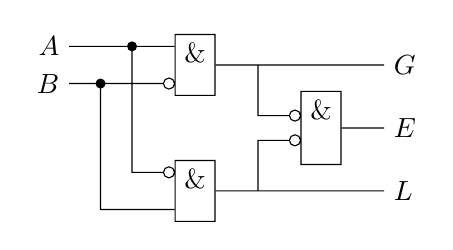
\begin{tikzpicture}[scale=.8]
            \node[and gate IEC, draw, logic gate inputs=nnni] at (0,0) (a1) {};
            \node[and gate IEC, draw, logic gate inputs=innn] at (0,-2) (a2) {};
            \node[and gate IEC, draw, logic gate inputs=ninin] at (2,-1) (o) {};
            \draw node (e1) at (-1,0) {}
            node (e2) at (-1.5,0) {}
            node (d) at (1,0) {}
            node (c) at (3,0) {}
            (a1.input 1)--(e1 |- a1.input 1)
            (a1.input 4)--(e2 |- a1.input 4)
            (a2.input 1)-|(e1 |- a1.input 1)
            (a2.input 4)-|(e2 |- a1.input 4)
            (e1 |- a1.input 1) to [short, *-] ++(-1,0) node[anchor=east] {$A$}
            (e2 |- a1.input 4) to [short, *-] ++(-0.5,0) node[anchor=east] {$B$}
            (a1.output)--(c|-a1.output) node[anchor=west]{$G$}
            (a2.output)--(c|-a2.output) node[anchor=west]{$L$}
            (o.output)--(c|-o.output) node[anchor=west]{$E$}
            (d|-a1.output) |- (o.input 2)
            (d|-a2.output) |- (o.input 4)
            ;
        \end{tikzpicture}
    \end{center}
    \paragraph{7.13}1). 输出保持之前的状态.\\
    2). $a$将变为$0$,$b$将变为$\overline{R}$.\\
    3). 是.

    \paragraph{7.14}
    储存器大小为$2^{64}\times4=2^{66}$字节,共储存$2^{66}\times8=2^{69}$位.
    \paragraph{7.15}
    $2^{14}\times\frac84=2^{15}$单元组.
    \paragraph{7.16}1). $A[1:0]=11_2,WE=1$\\
    2). 需要$\lceil\log_{2}10\rceil=4$条地址线,寻址能力没有发生变化.
\end{document}